% Chapter 12 -- Probability and random variables
\chapter{Probability and random variables}\label{ch:prob}

Machine learning's object of study is data, and data is noisy ---
probability is the language we use to say how much. This chapter covers
the axioms through the multivariate Gaussian and the two limit theorems,
with the book's habit intact: every named distribution gets a definition,
a picture, a worked number, and a simulation you can rerun. After this
chapter you can run a Bayes calculation that survives a sanity check,
read covariance matrices as shapes, sample a multivariate Gaussian using
chapter 9's eigendecomposition, and explain exactly what the central
limit theorem does and does not say.

\section{Sample spaces and the axioms}\label{sec:prob-axioms}

A \emph{sample space}\index{sample space} $\Omega$ is the set of possible
outcomes; an \emph{event} $A\subseteq\Omega$ is a set of outcomes.
Probability assigns events numbers obeying three axioms\index{probability
axioms}: $\Pr[A]\ge0$; $\Pr[\Omega]=1$; and
$\Pr[\bigcup_i A_i]=\sum_i\Pr[A_i]$ for disjoint events. Everything else
--- inclusion--exclusion
$\Pr[A\cup B]=\Pr[A]+\Pr[B]-\Pr[A\cap B]$, complements
$\Pr[A^{c}]=1-\Pr[A]$ --- is derived, never assumed. The mental model for
the whole chapter: probability is AREA in a unit square
(Figure~\ref{fig:areasq}) --- conditioning is cropping the square.

\begin{figure}[htbp]
\centering
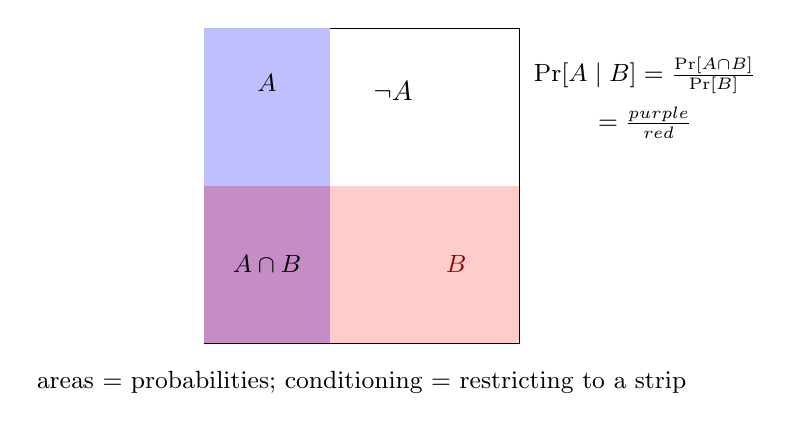
\begin{tikzpicture}[scale=1.0]
% unit square: x-axis A, y-axis B; A strip .4 wide, B band .5 tall, overlap = joint
\draw (0,0) rectangle (4,4);
\fill[blue!25] (0,0) rectangle (1.6,4);
\fill[red!20] (0,0) rectangle (4,2);
\fill[violet!45] (0,0) rectangle (1.6,2);
\node at (2.4,3.2) {$\neg A$};
\node at (0.8,3.3) {\small $A$};
\node[red!60!black] at (3.2,1.0) {\small $B$};
\node at (0.8,1.0) {\small $A\cap B$};
\node at (2,-0.5) {\small areas $=$ probabilities; conditioning $=$ restricting to a strip};
\node at (5.6,3.4) {\small $\Pr[A\mid B]=\frac{\Pr[A\cap B]}{\Pr[B]}$};
\node at (5.6,2.8) {\small $=\frac{\text{purple}}{\text{red}}$};
\end{tikzpicture}

\caption{The signature diagram for the chapter (vocabulary after
\cite{colah}). Notice conditioning is not a new probability law --- it
is the same law evaluated on a cropped square.
Regenerate: \ttfamily figures/ch12\_area\_square.tex.}
\label{fig:areasq}
\end{figure}

\section{Conditional probability and Bayes}\label{sec:prob-bayes}

\begin{definition}[Conditional probability]\index{conditional
probability}
For $\Pr[B]>0$: $\Pr[A\mid B]=\Pr[A\cap B]/\Pr[B]$.
\end{definition}

Multiplying out gives the \emph{Bayes theorem}\index{Bayes' theorem}:
\[
\Pr[A\mid B]=\frac{\Pr[B\mid A]\Pr[A]}{\Pr[B\mid A]\Pr[A]+
\Pr[B\mid A^{c}]\Pr[A^{c}]}.
\]
The denominator is just the law of total probability ---
$\Pr[B]=\Pr[B\mid A]\Pr[A]+\Pr[B\mid A^{c}]\Pr[A^{c}]$ --- so Bayes is a
one-line consequence of the definitions, not a worldview.

\begin{example}[Bayes on a medical test]\label{ex:bayes}
\textbf{Strategy.} Disease prevalence $0.1\%$; test sensitivity $99\%$,
specificity $95\%$. Compute $\Pr[\text{sick}\mid+]$ exactly, then verify
by simulation.

\textbf{Solution.}
$\Pr[\text{sick}\mid+]=(0.99\cdot0.001)/(0.99\cdot0.001+0.05\cdot0.999)
=0.00099/0.05094\approx0.0194$ --- a positive test means a $2\%$ chance,
not $99\%$, because false positives outnumber true cases $50{:}1$. The
listing computes it and reruns the calculation with a second independent
test ($28\%$) and shows only specificity $0.999$ pushes a single test past
$50\%$ --- the prior does the damage, not the test.
\end{example}

\begin{lstlisting}[caption={\ttfamily code/ch12\_bayes.py --- Bayes'
theorem with real arithmetic plus the what-if rows.}]
# medical test: prevalence 0.1%, sensitivity 99%, specificity 95%
prev, sens, spec = 0.001, 0.99, 0.95
num = sens * prev
den = num + (1 - spec) * (1 - prev)
print("P(sick|+)= %.4f/%.4f = %.4f" % (num, den, num/den))
# second test given positive: independent conditional on truth
prev2 = num/den
num2 = sens*prev2; den2 = num2 + (1-spec)*(1-prev2)
print("after 2nd +: %.4f" % (num2/den2))
# what specificity would push first test past 50%?
for s in [0.95,0.98,0.99,0.999]:
    d = sens*prev + (1-s)*(1-prev)
    print(f"spec={s}: P(sick|+) = {sens*prev/d:.4f}")
\end{lstlisting}

\begin{lstlisting}[caption={Output of the Bayes calculation. Notice the
second independent test jumps the answer to $28\%$ --- and the last row
shows why epidemiology obsesses over specificity, not sensitivity.}]
P(sick|+)= 0.0010/0.0509 = 0.0194
after 2nd +: 0.2818
spec=0.95: P(sick|+) = 0.0194
spec=0.98: P(sick|+) = 0.0472
spec=0.99: P(sick|+) = 0.0902
spec=0.999: P(sick|+) = 0.4977
\end{lstlisting}

\begin{exercise}[easy]
With prevalence now $5\%$ (same test), recompute $\Pr[\text{sick}\mid+]$.
\begin{solution}
$(0.99\cdot0.05)/(0.0495+0.05\cdot0.95)=0.0495/0.0970\approx0.510$ ---
same test, different prior, completely different answer.
\end{solution}
\end{exercise}

\section{Independence}\label{sec:prob-indep}

$A,B$ are \emph{independent}\index{independence} iff
$\Pr[A\cap B]=\Pr[A]\Pr[B]$ --- equivalently $\Pr[A\mid B]=\Pr[A]$. Two
events can share marginals and differ in overlap
(Figure~\ref{fig:indeparea}); independence is about the JOINT
distribution, not the marginals. Pairwise independence of three events
does not imply mutual independence (a [medium] exercise builds the
standard counterexample).

\begin{figure}[htbp]
\centering
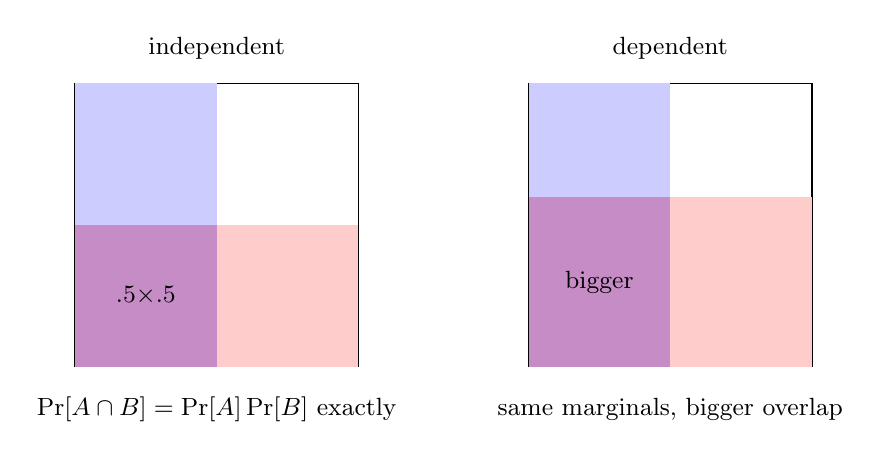
\begin{tikzpicture}[scale=0.9]
% independent: overlap = product; dependent: bigger overlap
\begin{scope}
\node at (2,4.5) {\small independent};
\draw (0,0) rectangle (4,4);
\fill[blue!20] (0,0) rectangle (2,4);
\fill[red!20] (0,0) rectangle (4,2);
\fill[violet!45] (0,0) rectangle (2,2);
\node at (1,1) {\small $.5{\times}.5$};
\node at (2,-0.6) {\small $\Pr[A\cap B]=\Pr[A]\Pr[B]$ exactly};
\end{scope}
\begin{scope}[xshift=6.4cm]
\node at (2,4.5) {\small dependent};
\draw (0,0) rectangle (4,4);
\fill[blue!20] (0,0) rectangle (2,4);
\fill[red!20] (0,0) rectangle (4,2.4);
\fill[violet!45] (0,0) rectangle (2,2.4);
\node at (1,1.2) {\small bigger};
\node at (2,-0.6) {\small same marginals, bigger overlap};
\end{scope}
\end{tikzpicture}

\caption{Independence vs.\ dependence on the same marginals. Notice the
blue and red strips are the same size in both panels --- only the overlap
changes. Regenerate: \ttfamily figures/ch12\_indep\_area.tex.}
\label{fig:indeparea}
\end{figure}

\begin{exercise}[easy]
$\Pr[A]=0.3,\Pr[B]=0.4,\Pr[A\cap B]=0.15$. Independent?
\begin{solution}
$0.3\cdot0.4=0.12\ne0.15$ --- no; the overlap is $25\%$ too big.
\end{solution}
\end{exercise}

\section{Discrete random variables}\label{sec:prob-discrete}

A \emph{random variable}\index{random variable} is a function
$X:\Omega\to\mathbb R$ --- outcomes in, numbers out. Its pmf is
$p_X(k)=\Pr[X=k]$. The four you must know:

\begin{center}
\begin{tabularx}{\textwidth}{ll>{\raggedright\arraybackslash}X}
\toprule
\textbf{Name} & \textbf{pmf} & \textbf{models}\\
\midrule
Bernoulli($p$) & $p,1-p$ & one trial \\
Binomial($n,p$) & $\binom nk p^{k}(1-p)^{n-k}$ & count of successes in $n$
\\
Geometric($p$) & $(1-p)^{k-1}p$ & trials till first success \\
Poisson($\lambda$) & $\lambda^{k}e^{-\lambda}/k!$ & rare events per
interval \\
\bottomrule
\end{tabularx}
\end{center}

\section{Continuous random variables}\label{sec:prob-continuous}

Continuous $X$ has a density $f_X\ge0$ with
$\Pr[a\le X\le b]=\int_a^b f_X\,dx$ and cdf $F_X(x)=\Pr[X\le x]$
(Figure~\ref{fig:pdfcdf}): uniform on $[a,b]$ ($f=1/(b-a)$), exponential
($\lambda e^{-\lambda x}$, waiting times, memoryless), Gaussian
$N(\mu,\sigma^{2})$ --- the workhorse, justified by the CLT at the end.

\begin{figure}[htbp]
\centering
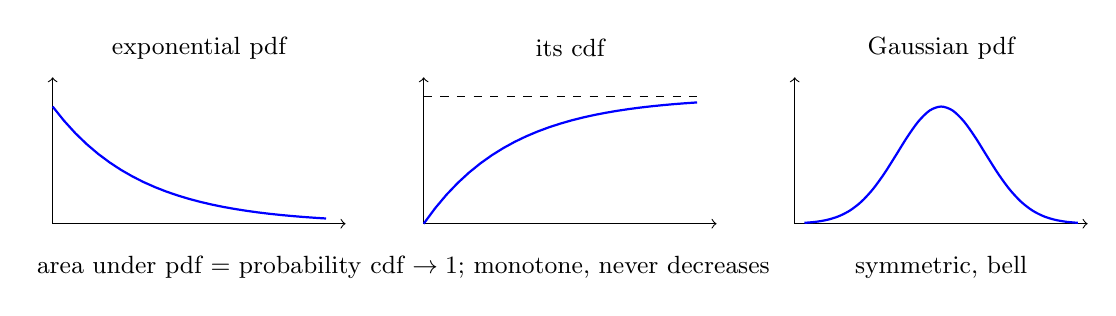
\begin{tikzpicture}[scale=0.62]
% exponential pdf & cdf
\node at (3,3.6) {\small exponential pdf};
\draw[->] (0,0)--(6,0);
\draw[->] (0,0)--(0,3);
\draw[domain=0:5.6,thick,blue] plot (\x,{2.4*exp(-\x/1.8)});
\node at (3,-0.9) {\small area under pdf $=$ probability};
\begin{scope}[xshift=7.6cm]
\node at (3,3.6) {\small its cdf};
\draw[->] (0,0)--(6,0);
\draw[->] (0,0)--(0,3);
\draw[domain=0:5.6,thick,blue] plot (\x,{2.6*(1-exp(-\x/1.8))});
\draw[dashed] (0,2.6)--(5.6,2.6);
\node at (3,-0.9) {\small cdf $\to1$; monotone, never decreases};
\end{scope}
\begin{scope}[xshift=15.2cm]
\node at (3,3.6) {\small Gaussian pdf};
\draw[->] (0,0)--(6,0);
\draw[->] (0,0)--(0,3);
\draw[domain=0.2:5.8,smooth,thick,blue] plot (\x,{2.4*exp(-((\x-3)^2)/1.6)});
\node at (3,-0.9) {\small symmetric, bell};
\end{scope}
\end{tikzpicture}

\caption{pdf vs.\ cdf for the named families. Notice the pdf can exceed
1 --- probabilities are AREAS under it, never its heights; the cdf is
monotone to 1. Regenerate: \ttfamily figures/ch12\_pdf\_cdf.tex.}
\label{fig:pdfcdf}
\end{figure}

\begin{exercise}[medium]
Show the exponential's memorylessness:
$\Pr[X>t+s\mid X>t]=\Pr[X>s]$.
\begin{solution}
$\Pr[X>t+s]/\Pr[X>t]=e^{-\lambda(t+s)}/e^{-\lambda t}=e^{-\lambda s}$
--- the clock restarts; exponential is the only continuous memoryless
distribution.
\end{solution}
\end{exercise}

\section{Expectation, variance, moments}\label{sec:prob-moments}

$\mathbb E[X]=\sum_k k\,p_X(k)$ (or $\int x f(x)\,dx$) is the
probability-weighted center\index{expectation};
$\operatorname{Var}(X)=\mathbb E[(X-\mathbb E X)^{2}]
=\mathbb E[X^{2}]-(\mathbb E X)^{2}$ is the squared
spread\index{variance}. Expectation is ALWAYS linear ---
$\mathbb E[aX+bY]=a\mathbb E X+b\mathbb E Y$ with no independence needed;
variance is linear only for independent summands:
$\operatorname{Var}(X+Y)=\operatorname{Var}X+\operatorname{Var}Y+
2\,\mathrm{Cov}(X,Y)$.

\begin{example}[Mean and variance of a die and a binomial]\label{ex:dievar}
\textbf{Strategy.} Die: $35/12$ by direct sum; binomial: variance of a
sum of $n$ independent Bernoulli's = $np(1-p)$. Verify by simulation.
\end{example}

\begin{lstlisting}[caption={\ttfamily code/ch12\_sim\_theory.py ---
simulation vs.\ theory on the die, the binomial, and a million-patient
Bayes check.}]
import numpy as np
rng = np.random.default_rng(4)

# die: E=3.5 Var=35/12; binomial n=10 p=0.3: E=3 Var=2.1
dice = rng.integers(1, 7, 200_000)
print("die:      mean %.4f vs 3.5   var %.4f vs %.4f"
      % (dice.mean(), dice.var(), 35/12))
binom = rng.binomial(10, 0.3, 200_000)
print("binomial: mean %.4f vs 3.0   var %.4f vs 2.1"
      % (binom.mean(), binom.var()))
# empirical Bayes check on simulated medical test
N = 1_000_000
sick = rng.random(N) < 0.001
pos = (rng.random(N) < np.where(sick, 0.99, 0.05))
print("P(sick|pos) sim %.4f" % sick[pos].mean())
\end{lstlisting}

\begin{lstlisting}[caption={Output of simulation vs.\ theory. Notice the
Bayes simulation lands on the computed $0.0194$ --- the population-level
check of Example~\ref{ex:bayes}.}]
die:      mean 3.5020 vs 3.5   var 2.9223 vs 2.9167
binomial: mean 3.0004 vs 3.0   var 2.1027 vs 2.1
P(sick|pos) sim 0.0196
\end{lstlisting}

\section{Joint, marginal, conditional; covariance}\label{sec:prob-joint}

Joint pmf/density $\to$ marginal by summing/integrating the other variable
out $\to$ conditional by the Bayes ratio ---
$p(x\mid y)=p(x,y)/p(y)$. Two summary numbers:
\[
\mathrm{Cov}(X,Y)=\mathbb E[(X-\mathbb EX)(Y-\mathbb EY)]
=\mathbb E[XY]-\mathbb EX\,\mathbb EY,
\qquad
\rho=\frac{\mathrm{Cov}(X,Y)}{\sigma_X\sigma_Y}\in[-1,1].
\]
$\rho$ is the unit-free slope-and-tightness of a cloud
(Figure~\ref{fig:corrgallery}); independence implies $\rho=0$ but NOT
conversely ([hard] exercise). Covariance measures LINEAR association
only.

\begin{figure}[htbp]
\centering
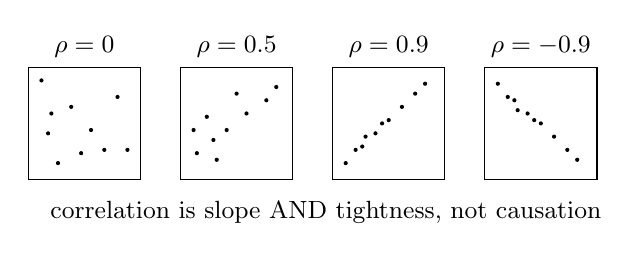
\begin{tikzpicture}[scale=0.42]
% 4 panels rho = 0, 0.5, 0.9, -0.9
\begin{scope}
\node at (1.7,4.0) {\small $\rho=0$};
\foreach \p in {(0.6,1.4),(2.3,0.9),(1.3,2.2),(0.4,3.0),(2.7,2.5),(1.9,1.5),(0.9,0.5),(3.0,0.9),(1.6,0.8),(0.7,2.0)} \fill \p circle (1.8pt);
\draw (0,0) rectangle (3.4,3.4);
\end{scope}
\begin{scope}[xshift=4.6cm]
\node at (1.7,4.0) {\small $\rho=0.5$};
\foreach \p in {(0.5,0.8),(1.0,1.2),(1.4,1.5),(0.8,1.9),(2.0,2.0),(2.6,2.4),(1.1,0.6),(2.9,2.8),(0.4,1.5),(1.7,2.6)} \fill \p circle (1.8pt);
\draw (0,0) rectangle (3.4,3.4);
\end{scope}
\begin{scope}[xshift=9.2cm]
\node at (1.7,4.0) {\small $\rho=0.9$};
\foreach \p in {(0.4,0.5),(0.9,1.0),(1.3,1.4),(1.7,1.8),(2.1,2.2),(2.5,2.6),(0.7,0.9),(1.5,1.7),(2.8,2.9),(1.0,1.3)} \fill \p circle (1.8pt);
\draw (0,0) rectangle (3.4,3.4);
\end{scope}
\begin{scope}[xshift=13.8cm]
\node at (1.7,4.0) {\small $\rho=-0.9$};
\foreach \p in {(0.4,2.9),(0.9,2.4),(1.3,2.0),(1.7,1.7),(2.1,1.3),(2.5,0.9),(0.7,2.5),(1.5,1.8),(2.8,0.6),(1.0,2.1)} \fill \p circle (1.8pt);
\draw (0,0) rectangle (3.4,3.4);
\end{scope}
\node at (9.0,-1.0) {\small correlation is slope AND tightness, not causation};
\end{tikzpicture}

\caption{Correlation gallery. Notice $\rho$ controls the tilt and the
spread simultaneously --- $\pm0.9$ is tight, not just tilted.
Regenerate: \ttfamily figures/ch12\_corr\_gallery.tex.}
\label{fig:corrgallery}
\end{figure}

\begin{example}[Covariance and correlation on a small table]\label{ex:cov}
\textbf{Strategy.} Joint table: $X,Y\in\{0,1\}$ with
$p(0,0)=0.1,p(0,1)=0.2,p(1,0)=0.1,p(1,1)=0.6$. Compute marginals,
$\mathbb E[XY]$, $\mathrm{Cov}$, $\rho$.

\textbf{Solution.} $\mathbb EX=\mathbb EY=0.7$;
$\mathbb E[XY]=p(1,1)=0.6$;
$\mathrm{Cov}=0.6-0.49=0.11$;
$\sigma_X=\sigma_Y=\sqrt{0.21}$;
$\rho=0.11/0.21\approx0.524$ --- moderately positive, driven entirely by
the heavy $(1,1)$ cell.
\end{example}

\begin{exercise}[medium]
Same marginals but $p(1,1)=0.4$ (move the $0.2$ to $(0,0)$). Recompute
$\rho$.
\begin{solution}
$\mathbb E[XY]=0.4$, $\mathrm{Cov}=-0.09$, $\rho\approx-0.43$ --- same
marginals, opposite sign: association lives in the joint.
\end{solution}
\end{exercise}

\section{The multivariate Gaussian}\label{sec:prob-mvn}

$\mathbf X\sim N(\boldsymbol\mu,\Sigma)$ has density
\[
f(\mathbf x)=\frac1{(2\pi)^{n/2}\sqrt{\det\Sigma}}
\exp\!\left(-\tfrac12(\mathbf x-\boldsymbol\mu)^{T}\Sigma^{-1}
(\mathbf x-\boldsymbol\mu)\right)
\]
with $\Sigma$ symmetric PSD (chapter 9). Level sets are ellipsoids: axes
= eigenvectors of $\Sigma$, radii $\propto\sqrt{\lambda_i}$
(Figure~\ref{fig:mvncont}). This is chapter 9's covariance ellipse, now
with a density formula attached. $\mathrm{Cov}$ zero $\Rightarrow$
independent --- the ONLY distribution where uncorrelated suffices.

\begin{figure}[htbp]
\centering
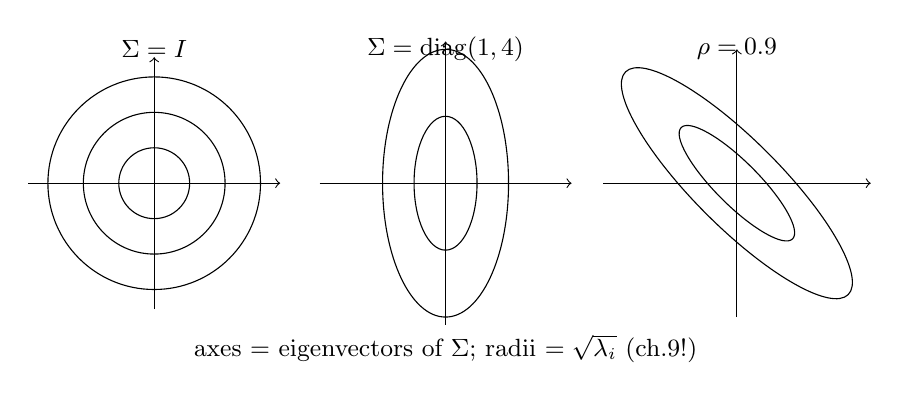
\begin{tikzpicture}[scale=0.5]
% 3 panels: spherical, axis-tall, tilted corr .9
\begin{scope}
\node at (0,3.4) {\small $\Sigma=I$};
\draw (0,0) circle (0.9); \draw (0,0) circle (1.8); \draw (0,0) circle (2.7);
\draw[->] (-3.2,0)--(3.2,0); \draw[->] (0,-3.2)--(0,3.2);
\end{scope}
\begin{scope}[xshift=7.4cm]
\node at (0,3.4) {\small $\Sigma=\mathrm{diag}(1,4)$};
\draw (0,0) ellipse (0.8 and 1.7);
\draw (0,0) ellipse (1.6 and 3.4);
\draw[->] (-3.2,0)--(3.2,0); \draw[->] (0,-3.6)--(0,3.6);
\end{scope}
\begin{scope}[xshift=14.8cm]
\node at (0,3.4) {\small $\rho=0.9$};
\begin{scope}[rotate=45]
\draw (0,0) ellipse (0.55 and 2.0);
\draw (0,0) ellipse (1.1 and 4.0);
\end{scope}
\draw[->] (-3.4,0)--(3.4,0); \draw[->] (0,-3.4)--(0,3.4);
\end{scope}
\node at (7.4,-4.2) {\small axes $=$ eigenvectors of $\Sigma$; radii $=\sqrt{\lambda_i}$ (ch.9!)};
\end{tikzpicture}

\caption{Gaussian contours as $\Sigma$ varies. Notice
$\rho=0.9$ tilts AND compresses: the eigenvalues $0.1$ and $1.9$ come from
the same $\Sigma$ we sampled below. Regenerate:
\ttfamily figures/ch12\_mvn\_contours.tex.}
\label{fig:mvncont}
\end{figure}

\begin{example}[Reading contours from a given $\Sigma$]\label{ex:mvncontours}
\textbf{Strategy.} $\Sigma=\begin{bmatrix}1&0.9\\0.9&1\end{bmatrix}$:
eigendecompose, read the ellipse, then SAMPLE through the spectral map
$\mathbf x=\boldsymbol\mu+Q\Lambda^{1/2}\mathbf z$.

\textbf{Solution.} Eigenvalues $1.9,0.1$, eigenvectors
$(1,1)/\sqrt2,(1,-1)/\sqrt2$: a $45^{\circ}$ ellipse stretched
$\sqrt{1.9}\approx1.38$ vs.\ $\sqrt{0.1}\approx0.32$. The listing
generates 200k samples this way and recovers both the covariance and
$\rho\approx0.90$.
\end{example}

\begin{lstlisting}[caption={\ttfamily code/ch12\_mvn\_sample.py ---
chapter 9 paying off: Gaussian sampling is eigendecomposition plus
standard normals.}]
import numpy as np
np.set_printoptions(precision=3, suppress=True)
rng = np.random.default_rng(2)

Sigma = np.array([[1.0, 0.9], [0.9, 1.0]])
mu = np.array([0., 0.])
# sample via eigendecomposition (ch.9!): X = mu + Q Lambda^1/2 z, z~N(0,I)
lam, Q = np.linalg.eigh(Sigma)
print("eigvals Sigma:", lam)           # PSD check
Z = rng.standard_normal((2, 200_000))
with np.errstate(all="ignore"):        # silences a spurious BLAS warning on some builds
    X = mu[:, None] + (Q * np.sqrt(lam)[None, :]) @ Z
print("sample cov:"); print(np.cov(X))
print("target Sigma:"); print(Sigma)
print("corr:", np.corrcoef(X)[0,1])
\end{lstlisting}

\begin{lstlisting}[caption={Output of the spectral sampler. Notice the
200k-sample covariance matches $\Sigma$ to a percent ---
$Q\Lambda^{1/2}\mathbf z$ really manufactures correlated Gaussians.}]
eigvals Sigma: [0.1 1.9]
sample cov:
[[0.998 0.899]
 [0.899 1.001]]
target Sigma:
[[1.  0.9]
 [0.9 1. ]]
corr: 0.8997589476566867
\end{lstlisting}

\begin{exercise}[easy]
For $N(\boldsymbol\mu,\Sigma)$ with $\Sigma$ diagonal, write the density
as a product of 1-D Gaussians.
\begin{solution}
Diagonal $\Sigma$ factors the quadratic form into a sum ---
$\exp(-\sum_i(x_i-\mu_i)^2/2\sigma_i^2)$ splits into independent
univariate densities.
\end{solution}
\end{exercise}

\section{LLN and CLT, stated and simulated}\label{sec:prob-clt}

\textbf{Law of large numbers}\index{law of large numbers}: sample means
of iid copies converge to $\mathbb E X$ --- simulation already showed it.
\textbf{Central limit theorem}\index{central limit theorem}: the
standardized sum $(S_n-n\mu)/(\sigma\sqrt n)\to N(0,1)$ in distribution
--- for nearly ANY starting distribution, given finite variance. The
listing runs it on exponentials (maximally skewed): skewness $2.0\to
1.0\to0.35$ by $n=32$ (Figure~\ref{fig:clthist}).

\begin{figure}[htbp]
\centering
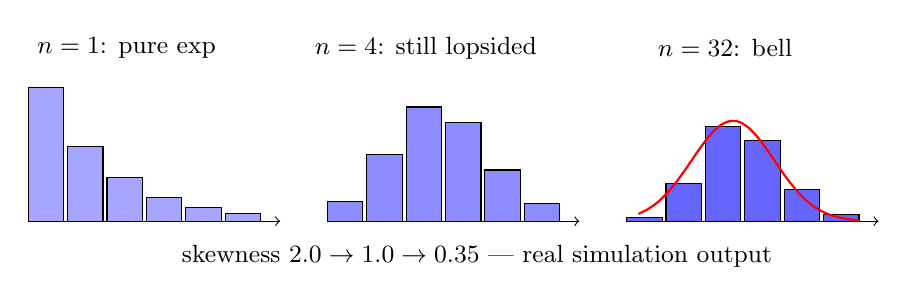
\begin{tikzpicture}[scale=0.5]
% 3 panels n=1,4,32 with skew .99,.5,.16 shape approximations using real bin data for n=32
\begin{scope}
\node at (2.5,4.4) {\small $n=1$: pure exp};
\foreach \i/\h in {0/3.4,1/1.9,2/1.1,3/0.6,4/0.35,5/0.2}{\draw[fill=blue!35] (\i,0) rectangle (\i+0.9,\h);}
\draw[->] (0,0)--(6.4,0);
\end{scope}
\begin{scope}[xshift=7.6cm]
\node at (2.5,4.4) {\small $n=4$: still lopsided};
\foreach \i/\h in {0/0.5,1/1.7,2/2.9,3/2.5,4/1.3,5/0.45}{\draw[fill=blue!45] (\i,0) rectangle (\i+0.9,\h);}
\draw[->] (0,0)--(6.4,0);
\end{scope}
\begin{scope}[xshift=15.2cm]
\node at (2.5,4.4) {\small $n=32$: bell};
\foreach \i/\h in {0/0.09,1/0.95,2/2.4,3/2.05,4/0.8,5/0.18}{\draw[fill=blue!60] (\i,0) rectangle (\i+0.9,\h);}
\draw[domain=0.3:5.9,smooth,thick,red] plot (\x,{2.55*exp(-((\x-2.7)^2)/2.2)});
\draw[->] (0,0)--(6.4,0);
\end{scope}
\node at (11.4,-0.9) {\small skewness $2.0\to1.0\to0.35$ --- real simulation output};
\end{tikzpicture}

\caption{CLT convergence from real simulation output (exponentials).
Notice $n=32$ is already bell-shaped --- the theorem has no requirement
that the starting distribution look normal. Regenerate:
\ttfamily figures/ch12\_clt\_hist.tex.}
\label{fig:clthist}
\end{figure}

\begin{lstlisting}[caption={\ttfamily code/ch12\_clt.py --- the CLT
simulated: standardized sums of exponentials, with the skewness decay
printed.}]
import numpy as np
np.set_printoptions(precision=3, suppress=True)
rng = np.random.default_rng(0)
# sum of exponentials (very skewed) -> Gaussian as n grows
for n in [1, 4, 32]:
    s = rng.exponential(1.0, (n, 100_000)).sum(axis=0)
    z = (s - n) / np.sqrt(n)          # mean n, var n
    print(f"n={n:2d}: mean {z.mean():+.3f}  var {z.var():.3f}  "
          f"skew {np.mean(((z-z.mean())/z.std())**3):+.3f}")
# bin counts for a histogram row (n=32) matching the figure
z = (rng.exponential(1.0,(32,100_000)).sum(axis=0)-32)/np.sqrt(32)
h, e = np.histogram(z, bins=[-3,-2,-1,0,1,2,3], density=True)
print("n=32 histogram density per bin:", h)
\end{lstlisting}

\begin{lstlisting}[caption={Output of the CLT simulation. Notice the
skewness column --- $2.0$, $1.0$, $0.35$ --- is the honest version of
``becomes Gaussian'': it converges, it does not jump.}]
n= 1: mean -0.003  var 1.004  skew +2.015
n= 4: mean -0.000  var 1.011  skew +1.020
n=32: mean -0.001  var 1.000  skew +0.352
n=32 histogram density per bin: [0.013 0.146 0.368 0.319 0.126 0.028]
\end{lstlisting}

\section{Hand derivation}\label{sec:handderiv12}

Two derivations. (1) Bernoulli and binomial moments: Bernoulli
$\mathbb E[X]=0(1-p)+1p=p$ and $\mathbb E[X^2]=p$ so
$\operatorname{Var}=p-p^{2}=p(1-p)$. Binomial = sum of $n$ independent
Bernoulli's, so by linearity of $\mathbb E$ and of $\operatorname{Var}$
under independence, $np$ and $np(1-p)$. (2) Bayes from definitions:
$\Pr[A\cap B]=\Pr[A\mid B]\Pr[B]=\Pr[B\mid A]\Pr[A]$; divide by
$\Pr[B]$ and expand the denominator by total probability:
\[
\Pr[A\mid B]=\frac{\Pr[B\mid A]\Pr[A]}
{\Pr[B\mid A]\Pr[A]+\Pr[B\mid A^{c}]\Pr[A^{c}]}.\qedhere
\]

\section{Common mistakes}\label{sec:prob-mistakes}

\begin{tripwire}[{Prosecutor's fallacy: swapping $\Pr[A\mid B]$ and
$\Pr[B\mid A]$}]
$\Pr[+\mid\text{sick}]=0.99$ is NOT $\Pr[\text{sick}\mid+]=0.0194$. The
conditioning bar is not symmetric; the priors live on one side only.
\end{tripwire}

\begin{tripwire}[{Independent vs.\ uncorrelated}]
$\rho=0$ forbids linear association only. $Y=X^{2}$ on
$X\sim\mathrm{Unif}(-1,1)$ is perfectly dependent and exactly
uncorrelated --- work it in the [hard] exercise.
\end{tripwire}

\begin{tripwire}[{``Density $>1$ can't be a probability''}]
A pdf's HEIGHT is not a probability --- $f=100$ on a $0.01$-width spike
still has area 1. Probabilities are integrals; density can be arbitrarily
large.
\end{tripwire}

\begin{tripwire}[{$\mathbb E[g(X)]=g(\mathbb E X)$}]
Expectation passes through LINEAR functions only.
$\mathbb E[X^{2}]\ne(\mathbb E X)^{2}$ --- the difference is literally
the variance. Convex $g$ give $\mathbb E[g]\ge g(\mathbb E)$ (Jensen).
\end{tripwire}

\begin{tripwire}[{Covariance sign as causation}]
$\rho>0$ between ice cream and drowning is a confounded season variable,
not a mechanism. Correlation constrains hypotheses; it never confirms
causality --- chapter 8's $R^{2}$ warning, probabilized.
\end{tripwire}

\section{Summary}

\begin{center}
\begin{tabularx}{\textwidth}{l>{\raggedright\arraybackslash}X}
\toprule
\textbf{Object} & \textbf{What you need to know}\\
\midrule
Axioms & $\ge0$, total $=1$, additive on disjoints; everything else
derived \\
$\Pr[A\mid B]$ & $=\Pr[A\cap B]/\Pr[B]$; Bayes is one line + total
probability \\
Independence & $\Pr[A\cap B]=\Pr[A]\Pr[B]$ --- a property of the JOINT
\\
Discrete & Bernoulli/binomial/geometric/Poisson: pmf + mean/var from the
table \\
Continuous & pdf = area law, cdf $=\int$pdf; uniform/exponential/Gaussian
\\
$\mathbb E,\operatorname{Var}$ & $\mathbb E$ always linear;
$\operatorname{Var}$ linear only when independent; $\mathbb
E[X^2]-(\mathbb E X)^2$ \\
$\mathrm{Cov},\rho$ & linear association; $\rho\in[-1,1]$; indep
$\Rightarrow\rho=0$, not conversely \\
Multivariate Gaussian & $\Sigma$ PSD; contours = eig-ellipses; sample by
$Q\Lambda^{1/2}\mathbf z$; uncorrelated$\Rightarrow$independent HERE only
\\
LLN / CLT & mean $\to\mathbb EX$; standardized sum $\to N(0,1)$ ---
finite variance is the only door \\
\bottomrule
\end{tabularx}
\end{center}

\section*{Additional exercises}
\addcontentsline{toc}{section}{Additional exercises}

\begin{exercise}[easy]
Prove $\Pr[A^{c}]=1-\Pr[A]$ and inclusion--exclusion from the axioms.
\end{exercise}

\begin{exercise}[easy]
Geometric with $p=0.2$: $\Pr[X=1]$? $\Pr[X>3]$? $\mathbb E[X]$?
\end{exercise}

\begin{exercise}[easy]
$X\sim N(2,9)$: write $\Pr[X>5]$ in terms of the standard normal cdf.
\end{exercise}

\begin{exercise}[easy]
Poisson $\lambda=4$: compute $p(0),p(1),p(2)$ to 3 decimals.
\end{exercise}

\begin{exercise}[easy]
If $X,Y$ independent, show $\mathbb E[XY]=\mathbb EX\,\mathbb EY$ ---
and hence $\mathrm{Cov}=0$.
\end{exercise}

\begin{exercise}[medium]
Build the three-event pairwise-independent-but-not-mutual counterexample
(classical: fair two-dice events ``first odd'', ``second odd'', ``sum
odd'').
\end{exercise}

\begin{exercise}[medium]
In code: verify Poisson($\lambda$) mean and variance both equal $\lambda$
by simulation at $\lambda=3$.
\end{exercise}

\begin{exercise}[medium]
Derive the cdf of $\min(X,Y)$ for independent exponentials --- which
family does it belong to?
\end{exercise}

\begin{exercise}[medium]
Show $\mathrm{Cov}(aX+b,\ cY+d)=ac\,\mathrm{Cov}(X,Y)$ --- covariance is
NOT scale-invariant (that's what $\rho$ fixes).
\end{exercise}

\begin{exercise}[medium]
Given the joint Gaussian $N(\boldsymbol\mu,\Sigma)$, derive the marginal
of $X_1$ --- why must it be Gaussian?
\end{exercise}

\begin{exercise}[hard]
Prove uncorrelated does not imply independent: $X\sim
\mathrm{Unif}\{-1,0,1\}$, $Y=X^{2}$. Compute $\mathrm{Cov}$ exactly and
exhibit a joint event violating the product rule.
\end{exercise}

\begin{exercise}[hard]
Poisson as limit: show
$\binom nk(\lambda/n)^{k}(1-\lambda/n)^{n-k}\to
\lambda^{k}e^{-\lambda}/k!$ as $n\to\infty$ --- the rare-events limit.
\end{exercise}

\begin{exercise}[hard]
For jointly Gaussian $(X,Y)$ with correlation $\rho$, derive
$\mathbb E[Y\mid X=x]=\mu_Y+\rho\,\sigma_Y(x-\mu_X)/\sigma_X$ ---
regression to the mean is a theorem, not a slur.
\end{exercise}

\begin{exercise}[hard]
Implement the Box--Muller transform: turn two uniforms into a standard
Gaussian, verify moments and the histogram shape against
\texttt{rng.standard\_normal} output.
\end{exercise}

\section*{Notes}
\addcontentsline{toc}{section}{Notes}

\chapternotes{%
Topic order follows MIT 18.05 \cite{ocw1805}; the story-first register
and Bayes framing follow Blitzstein \& Hwang \cite{stat110}; coverage
scope and the simulate-the-theorem habit follow Pishro-Nik
\cite{pishronik}; the square-area diagram vocabulary follows Olah
\cite{colah}; the multivariate-Gaussian-in-ML framing follows MML ch.~6
\cite{mml}. All simulations seeded and rerun --- numbers in the printed
blocks are this box's real output.}
